\documentclass[parskip]{komatufte}
\usepackage[subpreambles=false]{standalone}

%%%%%%%%%%%%%%%%%%%%%%%%%%%
% Silence warning messages
\usepackage{silence}
\WarningsOff[scrlayer-notecolumn]
\WarningsOff[biblatex]

%%%%%%%%%%%%%%%%%%%%
% Commenting

%\usepackage[author=Lyndon]{pdfcomment}
%\newcommand{\pdfcomment}[1]{} %ignore all comments

%\usepackage{todonotes}
%\newcommand{\pdfcomment}{\todo}


%%%%%%%%%%%%%%%%%%%%
% Tables
\usepackage{booktabs}

%%%%%%%%%%%%%%%%%%%
% Fonts
\usepackage{tgadventor} %sans
\usepackage{tgpagella}  %serif
\usepackage{inconsolata} %mono
\usepackage[T1]{fontenc}

\usepackage{microtype}
\usepackage[all]{nowidow}
%%%%%%%%%%%%%%%%%%%%%%%
% Styling
\setcounter{secnumdepth}{4}
\setcounter{tocdepth}{2}

\usepackage{placeins}



%%%%%%%%%%%%%%%%%%%
% Math
\usepackage{amsmath, amssymb, stmaryrd, mathtools}
\DeclareMathOperator*{\argmin}{argmin}
\DeclareMathOperator*{\argmax}{argmax}

\usepackage{xparse,xstring,etoolbox}
% crossref this against notation section
\newcommand{\vv}[1]{\tilde{#1}} % vector
\newcommand{\seq}[1]{\mathcal{#1}} % sequence
\newcommand{\set}[1]{\mathbb{#1}} % set

%%%%%%%%%
% Indexing/sequence indexing
\newcommand{\seqind}[2]{#1^{#2}} % seqence index
\newcommand{\ind}[2]{#1_{#2}} % indexed
\newcommand{\disamb}[2]{#1^{\mathrm{#2}}} %disambiguated

%% Smart indexing and naming
\newcommand{\ifupper}[3]{
    \normalexpandarg
	\exploregroups
	\StrCount{ABCDEFGHIJKLMNOPQRSTUVWXYZ}{#1}[\uppercount]
	\ifnumgreater{\uppercount}{0}{#2}{#3}
}

%smart index
\DeclareDocumentCommand{\ii}{u{_} m}{
	\ifupper{#1}%
	{% just a single uppercase character, i.e. a matrix
		  %make sure the index is the right length
		\StrCount{#2}{,}[\indcount]
		\ifnumgreater{\indcount}{0}
		{ % Got multiple indexes so all good
		 	\ind{#1}{#2}
		}
		{ % Only 1 index so grab the column
		 	\ind{#1}{{:,#2}}
		}
	}%
	{% Not just a single upper case character
		\ind{#1}{#2}
	}
}

\DeclareDocumentCommand{\nn}{u{_} m}{
	\seqind{#1}{#2}
}

\DeclareDocumentCommand{\dd}{u{_} m}{
	\disamb{#1}{#2}
}

% Index of a vector
\DeclareDocumentCommand{\iv}{u{_} m}{\ii{\vv #1}_{#2}}
\DeclareDocumentCommand{\dv}{u{_} m}{\dd{\vv #1}_{#2}}
\DeclareDocumentCommand{\nv}{u{_} m}{\nn{\vv #1}_{#2}}

%exp
\let\oldexp\exp
\renewcommand{\exp}[1]{\oldexp \left( #1 \right)}
\newcommand{\exptwo}[1]{\oldexp_2 \left( #1 \right)}

\newcommand{\softmax}{\mathrm{smax}}

\DeclareMathOperator*{\expectedop}{\mathbb{E}}
\DeclareDocumentCommand{\expected}{u{_} m}{
	\expectedop\limits_{\mathrlap{#2}}
}

%%%%%%%%%%%%%%%%
%Graphics
\usepackage{tikz}
\usetikzlibrary{positioning, fit,  shapes.geometric}
\usepackage{ifthen}
\usepackage{etoolbox}

\tikzset{
	backgroundcolor/.style ={fill=white},
	every node/.append style={
		minimum height=7mm,
	},
	labe/.append style={
		%Blue,
		align = center,
		backgroundcolor,
		fill opacity=0.6,
		text opacity=1,
		font={\footnotesize\itshape}	
	},
	layer/.append style={
		draw,
		align = center,
		minimum height=7mm,
	},
	tight/.append style={
		inner sep=0.2mm,
	},
	lookupbox/.append style={
		draw=none,
		append after command={
		       	[shorten <= -0.5\pgflinewidth]
		       	([shift={(-1.5\pgflinewidth,-0.5\pgflinewidth)}]\tikzlastnode.north east)
		       	edge([shift={( 0.5\pgflinewidth,-0.5\pgflinewidth)}]\tikzlastnode.north west) 
		       	([shift={( 0.5\pgflinewidth,-0.5\pgflinewidth)}]\tikzlastnode.north west)
		       	edge([shift={( 0.5\pgflinewidth,-1.5\pgflinewidth)}]\tikzlastnode.south west)            
		       	([shift={( -1.5\pgflinewidth,+0.5\pgflinewidth)}]\tikzlastnode.south east)
		       	edge([shift={(-1.5\pgflinewidth,-0.5\pgflinewidth)}]\tikzlastnode.north east)
		},
		inner sep=0.7mm,
		outer sep=0mm,
		minimum width=25mm
	}
}

\usepackage{pgfplots}
\pgfplotsset{compat=1.14}
\pgfplotsset{sideplot/.append style={
		width=\notescolwidth,
		domain=-10:10,
		samples=101,
		smooth,
		enlarge y limits={abs=2},
		axis lines=middle,
		xlabel  = $z$,
		ylabel  = $y$,
	},
	equ/.append style={
		color=blue,
		thick,
		mark=none
	}
}

% Function  For a plot 
% it  needs to be declared in preamble because of how \makenote* interacts with multiple files
\def\errorsurface(#1,#2){(0.5*#1 + 0.7*#2 + sin(deg(1.5*#1 + #2^2)))^2}


\usepackage{graphicx}
\graphicspath{{./figs/}, {./}, {./figs/chaptersentencerrepr/}, {./figs/chapterintromachinelearning/}, {./figs/chapterwordrepr/}}
\usepackage{adjustbox}


%%%%%%%%%%%%%%%%%%%
% Refs
\usepackage{cleveref}

\addbibresource{master.bib}

%%%%%%%%%%%%%%%%%%%%
% Formatting

% for examples from natural language space.
\newcommand{\natlang}[1]{\ifmmode \text{``\texttt{#1}''} \else {``\texttt{#1}''}\fi}
% \ifmmode ``trick'' from https://tex.stackexchange.com/a/15194/5834

%%%%%%%%%%%%%%%%%%%%%


\graphicspath{{./figs/chapterwordrepr}, {./}}


\begin{document}
\chapter{Word Representations}\label{sec:word-representations}
\begin{abstract}
Chapter 4: Word Representations (10 pages)
The core work that began to draw a lot of attention to this area.
This will cover crucial works such as Skip-Grams, CBOW, GLoVe, and of course the original neural probabilistic language model.
As well as more recent techniques based on matrix factorisations.
\end{abstract}

\aside[Word Vector or Word Embedding?]{Note that older literature in the area will use the term \emph{word~vector} to refer to representations from LDA and LSA etc. Whereas in a lot of newer work the term is used synonymously with \emph{word~embedding}.}
We begin the consideration of the representation of words using neural networks with work on language modeling
This is not the only place one could begin the consideration: the information retrieval (IR) models such as LDA and LSA based on word co-location would be the other obvious starting point.
However, as will be discussed there models are closer to the end point of of the chapter than the begin.
For the language modeling works, comes the contextual language model works such as skip-gram, which in turn lead to the post-neural network co-occurrence based works.
These model fundamentally are in fact more similar to the information retrieval co-location works than the language modeling from which we began.


\section{Representations for Language Modeling}

\aside[Random Variable Naming Convention]{We follow convention that capitalised $W_i$ is a random variable, and $w_i$ is a particular value which $W_i$ may take. Writing $P(\ldots W_i{=}w_i)$.
	Often though we will make uses of the abridged (abuse-of) notation and simply write $P(\ldots w_i)$, allowing the random variable to be implicitly given by the name of its value.
}

The language modeling task it to predict the next word given the words that came prior \pcite{rosenfeld2000two}.
For example, if a sentence begins \natlang{For lunch I will have a hot}, then there is a high probability that the next word will be \natlang{dog} or \natlang{meal},
and lower probabilities of words such as \natlang{day} or \natlang{are}.
Mathematically it is formulated: 
\begin{equation}\label{equ:langmodel}
	P(W_n{=}w_i \mid W_{i-1}{=}w_{i-1}, \ldots, W_1{=}w_1)
\end{equation}
or to use the compact notation 
\begin{equation}\label{equ:langmodelcompact}
P(w_i \mid w_{i-1}, \ldots, w_1)
\end{equation}
$P(w_i \mid \natlang{hot}, \natlang{a}, \natlang{want}, \natlang{I}, \natlang{lunch}, \natlang{For})$.
The task is to find the probabilities for the various words that $w_i$ could represent.

\aside[Google n-gram corpora]{Google has created several very large scale corpora of 1,2,3,4, and 5-grams from over $10^{11}$ words.
Including the 2006 Web corpus from the public internet (Available for fees at \url{https://catalog.ldc.upenn.edu/LDC2006T13}),
and the 2010-2012 Books corpus made words from the Google Books project (available freely from \url{https://books.google.com/ngrams/datasets}), as described in \textcite{lin2012syntactic}.
These very large corpora also used outside of statistical language modeling by corpus linguists investigating the use of language.
}

  
The classical approach is trigram statistical language modeling.
In this, the number of word triples in a corpus is counted,
then given the previous two words, the next is predicted based on those counts.
This is making the Markov assumption that the next state depends only on the current state,
and that that state can be described by previous two words.
Under this assumption \Cref{equ:langmodelcompact} becomes:
\begin{equation}\label{equ:trigramlangmodel}
P(w_i \mid w_{i-1}, \ldots, w_1) = P(w_i \mid w_{i-1}, w_{i-2})
\end{equation}
More generally, one can use $n$-gram language model where for any value if $n$,
this is simply a matter of defining the Markov state to contain fewer or greater numbers of previous words than in the trigram case.

This Markov assumption is, of-course, an approximation.
In the previous example, a trigram language model is finding $P(w_i \mid \natlang{hot}, \natlang{a})$.
It can be seen that the approximation has lost key information.
Based only on the previous 2 words the next word $w_i$ could now reasonably be \natlang{day}, but the sentence: \natlang{For lunch I will have a hot day} makes no sense.
However, the Markov assumption in using $n$-grams is required in order to make the problem tractable -- otherwise an unbound amount of information would need to be stored. 

They key issue with n-gram language models in that in training them there is a data-sparsity problem.
Most combinations of words occur very rarely \pcite{ha2009extending}.
It is thus hard to estimate their occurrence probability.
Combinations of words that do not occur in the model is derived from as naturally given a probability of zero.
This is unlikely to be true though -- it is simply a matter of rare words never occurring together in a finite corpus.
Several approaches have been taken to handle this.
Simplest is add-one smoothing which adds an extra pseudo-observation of every combination of terms.
In common use is are various back-off methods \pcite{katz1987estimation,kneser1995improved} which use the bigram probabilities to estimate the probabilities of unseen trigrams.
%
\aside{An extended look at classical techniques in statistical language modelling can be found in \textcite{DBLP:journals/corr/cs-CL-0108005}}
%
However, these methods are merely clever statistical tricks -- ways to reassign probability mass after the fact to leave some left-over for unseen cases.
Back-off is smarter than add-one smoothing, as it portions the probability fairly based of the $n{-}1$-gram probability.
Better still would be a method which can learn to see the common-role of words.
By looking at the fragment: \natlang{For lunch I want a hot}, any reader knows that the next word is most likely going to be a food.
We know this for the same reason we know the next word in \natlang{For elevenses  I had a cold ...} is also going to be a food.
Even though \natlang{elevenses} is a vary rare word, we know from the context that it is a meal (more on this later), and we know it shares other traits with meals, and similarly \natlang{have} / \natlang{had}, and \natlang{hot} / \natlang{cold}.
These traits influence the words that can occur after them.
Thus the motivation is for a language modeling method that use these common properties of the words in the language modeling.
We need representation that holds this information.


\tcite{NPLM} presents a method that uses neural network representations in a language model, where this representations implicitly learn the crucial traits of words.
Capturing the trait information in the representation of a word for use in language modeling is not an idea exclusive to neural network approaches.
Almost a decade earlier was the clustering work of  \tcite{brown1992class}.
The method of \tcite{NPLM} however, implicitly learns this information into a neural network bases representation in during the training for the language modeling task.

To understand the neural probabilistic language model, first consider a simplified neural trigram language model.
This model is a simplification of that introduces by \tcite{NPLM}, it forms the basis of several models and introduces the most important idea in neural language representations: that of training a vector representation of a word using a lookup table to map a discrete word to a vector that becomes the first layer of the network.



\aside[Lookup word embeddings: Hashmap or Array?]{
The question is purely one of implementation.
Theoretically we do not care if the implementation using a String to Vector dictionary (eg a Hashmap), or an 2D Array which is indexed into via an integer index representing the word, to retrieve a column.
In tokenization of the source text it is common to transform all the words into integers, so as to save memory, especially if the tokenization does not make use of string interning.
At that point it makes sense to work with a Array.
For our purposes we will treat the word $w_i$ as if it were an integer index, though thinking of it as a string index into a hashmap changes little in the logic.
}

\aside[One-hot product or Indexed-lookup]{
In some works you may see the process of retrieving the word vector from an Matrix of word vectors described as a one-hot multiplication.
That is to say for a word represented by the index $i$,
for $e_i$ the one-hot vector with a 1 in the $i$th position,
and for $C$ the table of word embeddings.
one can write  $Ce_i$.
We will write $C_i$ and refer to this as looking up the word vector from the $i$th column.
Of-course $C_i=Ce_i$, however in practical implementation the performance ramification are huge.
A matrix column indexing is a $O(1)$ operation (for column major languages),
where as a dense matrix-vector product is $O(n^2)$.
%
The one-hot product can be used in a pinch to support using embeddings in neural network toolkits that do not support lookup/embedding layers,
however we strongly suggest that if your toolkit does not support lookup/embedding layers then it is unsuitable for use in NLP applications.
}

The trigram neural probabilistic network is defined by:
%
\begin{multline}
P(w_i \mid w_{i-1}, w_{i-2}) = \\
s_{max}\left(U_2 \: \varphi\left(U_1\left[C_{w_{i-1}}; C_{w_{i-2}}\right] + b_1\right)+b_2\right)
\end{multline}
%
where $U_1,\: U_2,\: b_1,\: b_2$ are the weight matrices and biases of the network, and $C_{w_{i-1}}$ and $C_{w_{i-2}}$ are the looked-up word embedding for the previous two words, from the embedding table $C$.
We write $\left[v_1; v_2\right]$ as a notational convenience for the concatenation of vectors $v_1$ and $v_2$.
The network is shown diagrammatically in \Cref{fig:trigram-neural-language-model}

\begin{figure}
	\centering
	\documentclass{article}

\usepackage{tikz}
\usetikzlibrary{positioning, fit,  shapes.geometric}
\usepackage{ifthen}
\usepackage{etoolbox}

\tikzset{
	backgroundcolor/.style ={fill=white},
	every node/.append style={
		minimum height=7mm,
	},
	labe/.append style={
		%Blue,
		align = center,
		backgroundcolor,
		fill opacity=0.6,
		text opacity=1,
		font={\footnotesize\itshape}	
	},
	layer/.append style={
		draw,
		align = center,
		minimum height=7mm,
	},
	tight/.append style={
		inner sep=0.2mm,
	},
	lookupbox/.append style={
		draw=none,
		append after command={
		       	[shorten <= -0.5\pgflinewidth]
		       	([shift={(-1.5\pgflinewidth,-0.5\pgflinewidth)}]\tikzlastnode.north east)
		       	edge([shift={( 0.5\pgflinewidth,-0.5\pgflinewidth)}]\tikzlastnode.north west) 
		       	([shift={( 0.5\pgflinewidth,-0.5\pgflinewidth)}]\tikzlastnode.north west)
		       	edge([shift={( 0.5\pgflinewidth,-1.5\pgflinewidth)}]\tikzlastnode.south west)            
		       	([shift={( -1.5\pgflinewidth,+0.5\pgflinewidth)}]\tikzlastnode.south east)
		       	edge([shift={(-1.5\pgflinewidth,-0.5\pgflinewidth)}]\tikzlastnode.north east)
		},
		inner sep=0.7mm,
		outer sep=0mm,
		minimum width=25mm
	}
}

\begin{document}

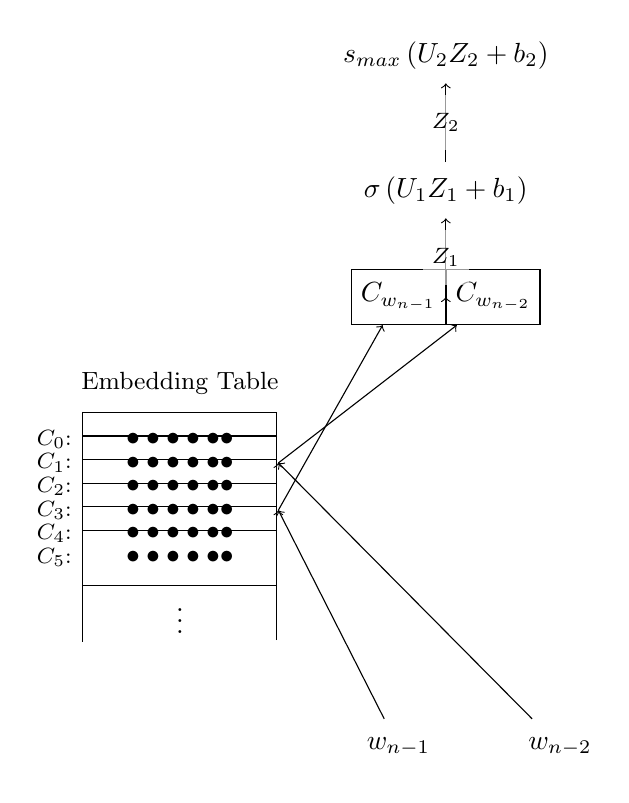
\begin{tikzpicture}[]


\node(w1) {$w_{n-1}$};
\node(w2)[right = of w1] {$w_{n-2}$};


\node(Cn)[lookupbox, above left=of w1] {$\vdots$};
\def\tblmax{6}
\foreach \ii in {1,...,\tblmax} {
	\pgfmathsetmacro\pos{(\ii - 1) * 3 };
	\pgfmathtruncatemacro\jj{(\tblmax -\ii)};
	
	\node(C\ii)[lookupbox, above = \pos mm of Cn]{$\bullet\bullet\bullet\bullet\bullet\bullet$};
	\node(Clbl\ii)[left = 0mm of C\ii]{\footnotesize $C_\jj$:};
};
\node(C)[above = 0mm of C\tblmax] {\small Embedding Table};



\node(concat1)[layer, above = 5 of w1]{$C_{w_{n-1}}$};
\node(concat2)[layer, right = 0 of concat1]{$C_{w_{n-2}}$};

\draw[->] (w1) edge (C3.east);
\draw[->]  (C3.east) edge (concat1);
\draw[->] (w2) edge (C5.east);
\draw[->]  (C5.east) edge (concat2);

\node(L1)[above = of concat1.east]{$\sigma\left(U_1Z_1 + b_1\right)$};
\draw[->]  (concat1.east) edge node[labe]{$Z_1$} (L1);

\node(L2)[above = of L1]{$s_{max}\left(U_2 Z_2 + b_2\right)$};
\draw[->]  (L1) edge node[labe]{$Z_2$} (L2);

\end{tikzpicture}

\end{document} 
	\caption{\label{fig:trigram-neural-language-model} Neural Trigram Language Model}
\end{figure}

In the neural trigram language model, each of the previous two words is used to look-up a vector from the Embedding Table matrix.
These are then concatenated to give a dense, continuous-space input to the above hidden layer.
The output layer is a softmax layer, it gives the probabilities for each word in the vocabulary, one of which corresponds to $w_i$ the word being evaluated.

The word embeddings are trained, via the normal neural network method, along with the network weights and biases.
This allows the embeddings of words which predict the same future word to move to be near each other in vector space.
It also allows the hidden layer to learn to associate information with regions of the embedding space.
This thus allows for information sharing between words.
If two words vectors are close together because they mostly predict the same future words, then that area of space is a associated with predicting those words.
Thus for cases where there are some words which never co-occur in the training set, but for which the nearby word does co-occur with, then because the knowledge is associated with that region of space, the model predicts that there is a higher-than-zero chance of the first word co-occurring with the unseen word.
This is a fuzzy and nonlinear relationship, with varying degrees of closeness resulting in (and from) varying levels of exception of the words sharing co-occurring predicted words.


\tcite{NPLM} is a more advanced version of the neural language model discussed.
Rather than being a trigram language model, it is an $n$-gram language model, where $n$ is a hyper-parameter of the model.
The knowledge sharing allows the data-sparsity issues to be ameliorated, thus allowing for $n>3$.
%
\aside{\textcite{schwenk2004efficient} suggests using only a subset of the vocabulary as options for the output, while allowing the full vocabulary in the input space -- with a fallback to classical language models for the missed words.
	This decreases the size of the softmax output layer, substantially decreasing the network evaluation and training time.
	This technique is now largely eclipsed by hierarchical softmax etc. discussed later in this chapter.
}
%
Bengio et. al. investigates values for $n$ of 3, 5 and 6.
The network used in their work also was marginally more complex, as shown in \Cref{fig:neural-language-model} and in the following equation:
\begin{align}
P(w_i & \mid w_{i-1}, w_{i-2}) = s_{max}( \nonumber
\\  & \quad U_3 \left[ C_{w_{i-1}};...; C_{w_{i-n}}\right] \nonumber
\\  & + U_2 \: \varphi\left( U_1\left[C_{w_{i-1}};...; C_{w_{i-n}} \right] + b_1\right) \nonumber
\\  & +b_2)
\end{align}

It includes a layer-bypass, which is primarily present only as connivance to aid in the learning.
It allowing the input to directly effect the output without being mediated by the shared hidden layer.
This layer-bypass is a unusual feature, not present in future works deriving from this, such as \tcite{schwenk2004efficient} which presents a bag of tricks to minimize training time. 





This is the network which begins the notions of using neural networks with vector representations of words.
Bengio et. al. focused on the use of the of sliding window of previous words -- much like the traditional n-grams.
At each time-step the window is advanced forward and the next word predicted based on that shifted context of prior words.
They do very briefly mention that an RNN could be used in its place.

\begin{figure}
	\centering
	\documentclass{article}

\usepackage{tikz}
\usetikzlibrary{positioning, fit,  shapes.geometric}
\usepackage{ifthen}
\usepackage{etoolbox}

\tikzset{
	backgroundcolor/.style ={fill=white},
	every node/.append style={
		minimum height=7mm,
	},
	labe/.append style={
		%Blue,
		align = center,
		backgroundcolor,
		fill opacity=0.6,
		text opacity=1,
		font={\footnotesize\itshape}	
	},
	layer/.append style={
		draw,
		align = center,
		minimum height=7mm,
	},
	tight/.append style={
		inner sep=0.2mm,
	},
	lookupbox/.append style={
		draw=none,
		append after command={
		       	[shorten <= -0.5\pgflinewidth]
		       	([shift={(-1.5\pgflinewidth,-0.5\pgflinewidth)}]\tikzlastnode.north east)
		       	edge([shift={( 0.5\pgflinewidth,-0.5\pgflinewidth)}]\tikzlastnode.north west) 
		       	([shift={( 0.5\pgflinewidth,-0.5\pgflinewidth)}]\tikzlastnode.north west)
		       	edge([shift={( 0.5\pgflinewidth,-1.5\pgflinewidth)}]\tikzlastnode.south west)            
		       	([shift={( -1.5\pgflinewidth,+0.5\pgflinewidth)}]\tikzlastnode.south east)
		       	edge([shift={(-1.5\pgflinewidth,-0.5\pgflinewidth)}]\tikzlastnode.north east)
		},
		inner sep=0.7mm,
		outer sep=0mm,
		minimum width=25mm
	}
}

\begin{document}

\begin{tikzpicture}[]


\node(w1) {$\n w_{i-1}$};
\node(w2)[right = 0mm  of w1] {$\n w_{i-2}$};
\node(w3)[right = 0mm of w2] {$\ldots$};
\node(w4)[right = 0mm of w3] {$\n w_{i-n}$};


\node(Cn)[lookupbox, above left=of w1] {$\vdots$};
\def\tblmax{6}
\foreach \ii in {1,...,\tblmax} {
	\pgfmathsetmacro\pos{(\ii - 1) * 3 };
	\pgfmathtruncatemacro\jj{(\tblmax -\ii)};
	
	\node(C\ii)[lookupbox, above = \pos mm of Cn]{$\bullet\bullet\bullet\bullet\bullet\bullet$};
	\node(Clbl\ii)[left = 0mm of C\ii]{\footnotesize $\i C_\jj$:};
};
\node(C)[above = 0mm of C\tblmax] {\small \textsc{Embedding Table}};


\node(concat1)[layer, above = 5 of w1]{$\i C_{\n w_{i-1}}$};
\node(concat2)[layer, right = 0 of concat1]{$\i C_{\n w_{i-2}}$};
\node(concat3)[layer, right = 0 of concat2]{$\quad\ldots\quad$};
\node(concat4)[layer, right = 0 of concat3]{$\i C_{\n w_{i-n}}$};
 
\draw[->] (w1) edge (C3.east);
\draw[->]  (C3.east) edge (concat1.south);
\draw[->] (w2) edge (C5.east);
\draw[->]  (C5.east) edge (concat2.south);
\draw[->] (w4) edge (C5.east);
\draw[->]  (C5.east) edge (concat4.south);

\node(L1)[layer, above = of concat2.north east]{$\varphi\left(\d U_{hid}\dv z_{embs} + \v b\right)$};
\draw[->]  (concat2.north east) -- node[labe]{$\dv z_{embs}$} (L1);


\node(L2)[layer, above = of L1]{$s_{max}\left(V \dv z_{hid} +\d U_{bypass} \dv z_{embs}+ \v k\right)$};
\draw[->]  (L1) edge node[labe]{$\dv z_{hid}$} (L2); 
\draw[->, bend right] (concat2.north east)  to[bend right=45, min distance=25 mm] (L2);


\node(out)[above = of L2]{$P(\n w_i \mid \n w_{i-1}, \n w_{i-2}, \ldots, \n w_{i-n})$};
\draw[->] (L2) edge (out);


\end{tikzpicture}

\end{document} 
	\caption{\label{fig:neural-language-model} Neural Probabilistic Language Model}
\end{figure}


\subsection{RNN Language Models}
In \tcite{mikolov2010recurrent} an RNN is for a language model.
\aside[Differences in formulation]{
The network and equations shown here may seem different to those presented in \textcite{mikolov2010recurrent}.
However they are mathematically identical.
The apparent difference is simply the choice between considering embeddings as a look-up, or as a one-hot multiplication.
}
To be precise, an Elman network is used.
In this form of RNN, the output of hidden layer in the previous time-step is appended as an additional input.
Using an RNN eliminates the sliding window of earlier language models.
Instead, the context information is stored in the state that is passed forward.




\begin{equation}
%
%
\end{equation}

\begin{figure}
	\centering
	\documentclass{article}

\usepackage{tikz}
\usetikzlibrary{positioning, fit,  shapes.geometric}
\usepackage{ifthen}
\usepackage{etoolbox}

\tikzset{
	backgroundcolor/.style ={fill=white},
	every node/.append style={
		minimum height=7mm,
	},
	labe/.append style={
		%Blue,
		align = center,
		backgroundcolor,
		fill opacity=0.6,
		text opacity=1,
		font={\footnotesize\itshape}	
	},
	layer/.append style={
		draw,
		align = center,
		minimum height=7mm,
	},
	tight/.append style={
		inner sep=0.2mm,
	},
	lookupbox/.append style={
		draw=none,
		append after command={
		       	[shorten <= -0.5\pgflinewidth]
		       	([shift={(-1.5\pgflinewidth,-0.5\pgflinewidth)}]\tikzlastnode.north east)
		       	edge([shift={( 0.5\pgflinewidth,-0.5\pgflinewidth)}]\tikzlastnode.north west) 
		       	([shift={( 0.5\pgflinewidth,-0.5\pgflinewidth)}]\tikzlastnode.north west)
		       	edge([shift={( 0.5\pgflinewidth,-1.5\pgflinewidth)}]\tikzlastnode.south west)            
		       	([shift={( -1.5\pgflinewidth,+0.5\pgflinewidth)}]\tikzlastnode.south east)
		       	edge([shift={(-1.5\pgflinewidth,-0.5\pgflinewidth)}]\tikzlastnode.north east)
		},
		inner sep=0.7mm,
		outer sep=0mm,
		minimum width=25mm
	}
}

\begin{document}

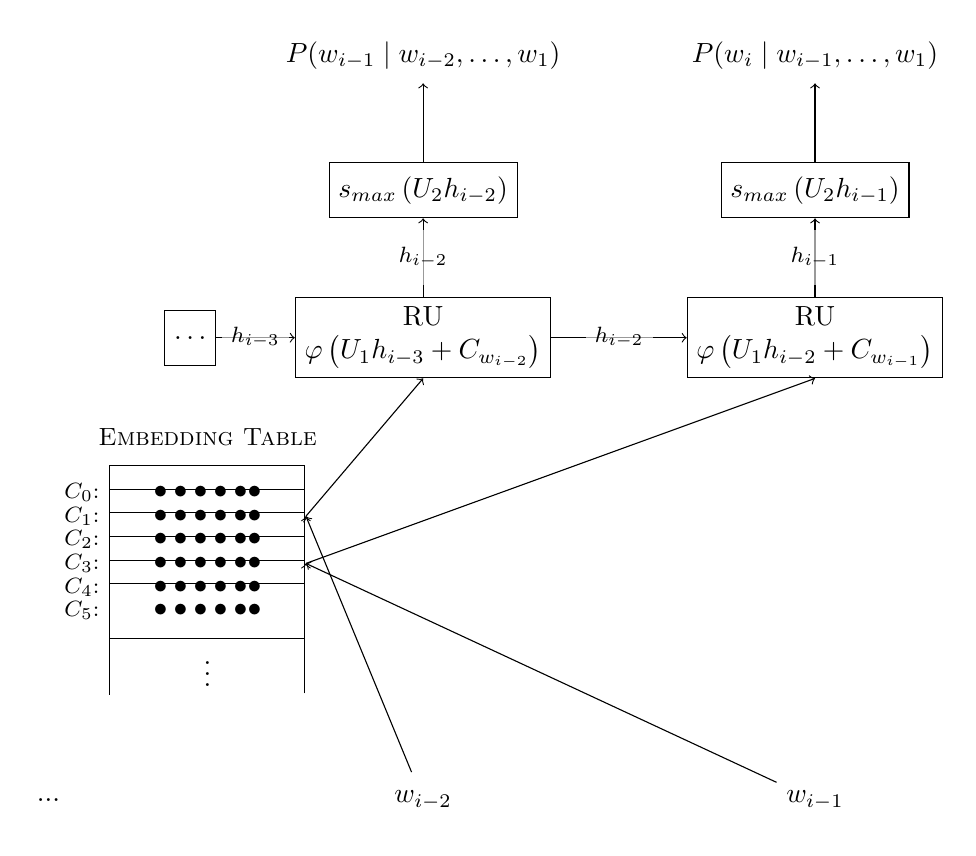
\begin{tikzpicture}[]

\newcommand{\hsep}{4}
\newcommand{\vtablesep}{5}

\node(w1) {$w_{i-1}$};
\node(w2)[left = \hsep of w1] {$w_{i-2}$};
\node(w3)[left = \hsep of w2] {$...$};


\node(Cn)[lookupbox, above left=of w2] {$\vdots$};
\def\tblmax{6}
\foreach \ii in {1,...,\tblmax} {
	\pgfmathsetmacro\pos{(\ii - 1) * 3 };
	\pgfmathtruncatemacro\jj{(\tblmax -\ii)};
	
	\node(C\ii)[lookupbox, above = \pos mm of Cn]{$\bullet\bullet\bullet\bullet\bullet\bullet$};
	\node(Clbl\ii)[left = 0mm of C\ii]{\footnotesize $C_\jj$:};
};
\node(C)[above = 0mm of C\tblmax] {\small \textsc{Embedding Table}};

\node(L11)[layer, above = \vtablesep of w1]{RU\\$\varphi\left( U_1h_{i-2}  +  C_{w_{i-1}}\right)$};
\node(L21)[layer, above = of L11]{$s_{max}\left(U_2 h_{i-1}\right)$};
\draw[->]  (L11) edge node[labe]{$h_{i-1}$} (L21);
\node(out1)[above = of L21]{$P(w_i \mid w_{i-1}, \ldots,  w_1)$};
\draw[->] (L21) edge (out1);

\node(L12)[layer, above = \vtablesep of w2]{RU\\$\varphi\left( U_1h_{i-3}  +  C_{w_{i-2}}\right)$};
\node(L22)[layer, above = of L12]{$s_{max}\left(U_2 h_{i-2} \right)$};
\draw[->]  (L12) edge node[labe]{$h_{i-2}$} (L22);
\node(out2)[above = of L22]{$P(w_{i-1} \mid w_{i-2}, \ldots,  w_1)$};
\draw[->] (L22) edge (out2);
\draw[->]  (L12) edge node[labe]{$h_{i-2}$} (L11);

\node(L13)[layer, left = of L12] {$\ldots$};
\draw[->]  (L13) edge node[labe]{$h_{i-3}$} (L12);


\draw[->] (w1) edge (C3.east);
\draw[->]  (C3.east) edge (L11.south);
\draw[->] (w2) edge (C5.east);
\draw[->]  (C5.east) edge (L12.south);


\end{tikzpicture}

\end{document} 
	\caption{\label{fig:neural-language-model} RNN Language Model}
\end{figure}


\tcite{mikolov2011RnnLM}
\tcite{mikolov2011trainingstrategies}

\section{Contextual Language Modeling}

\tcite{mikolov2012contextRNNLM} a

\subsection{CBOW}
\tcite{mikolov2013linguisticsubstructures}
\tcite{mikolovSkip}
 
\subsection{SkipGram}
\tcite{mikolov2013linguisticsubstructures}
\tcite{mikolovSkip} a

\aside[Pretrained Word-Embeddings]{
Pretrained Word Embeddings are available for most models discussed here.
There trained on a lot more data than most people have access too.
It can be useful to substitute word embeddings are a representation in most systems.}

\subsection{Glove}

General consensus has emerged that Glove performs marginally worse than skip-grams

\subsection{What ever it is that people do instead now that is basically SVD on colloations}


\section{Natural Language Applications -- beyond language modeling}
While statistical language models are useful, they are of-course in no way the be-all and end-all of natural language processing.
Simultaneously with the developments around representations for the language modelling tasks, work was being done on solving other NLP problems using similar techniques.

\tcite{collobert2008unified}

\tcite{turian2010word}





\clearnotecolumn[notes]

\end{document}
